% Presenter 1: slides 1--6, 0:00--4:00. Presenter 2: slides 7--12, 4:00--8:00.
\section{Introduction}

% 2: 0:10--0:50. Reveals: intro/statistics -> heat drivers -> goal -> appendix link.
\begin{frame}[more-space]{Introduction\enspace|\enspace Why a thermal digital twin?}
  \par\vfill
  \small AI training and deployment rely on data centers.%
  \begin{tikzpicture}[remember picture,overlay]
    \node<4->[anchor=south east,rounded corners=1mm,
      fill=rwth-blue-100,text=white,inner xsep=3mm,inner ysep=2mm,
      font=\small\bfseries]
      at ([xshift=-4mm,yshift=18mm]current page.south east)
      {Full plan in \hyperlink{backup-index}{\textcolor{white}{\underline{Appendix}}}};
  \end{tikzpicture}%
  \par\vfill
  \begin{columns}[T,onlytextwidth]
    \column{0.31\textwidth}\datametric{1.5\,\%}{World electricity used by data centers in 2024}
    \column{0.31\textwidth}\datametric{12\,\% / year}{Growth over the preceding five years}
    \column{0.31\textwidth}\datametric{7 to >30\,\%}{Cooling share, depending on facility type}
  \end{columns}
  \par\vfill
  \begin{uncoverenv}<2->
  \begin{beamercolorbox}[sep=2mm,wd=\textwidth]{data panel}
    \centering
    \begin{tikzpicture}[font=\small]
      \node[inner sep=0pt] (drivers) {%
        \begin{minipage}{40mm}
          \small
          \begin{itemize}
            \item More CPU power
            \item Warmer inlet air
            \item Less air flow or fan power
          \end{itemize}
        \end{minipage}%
      };
      \node[right=8mm of drivers,rounded corners=1.5mm,
        draw=rwth-blue-100!35,fill=white,inner sep=3mm,
        text=rwth-blue-100] (effect) {\textbf{hotter CPUs}};
      \draw[->,thick,rwth-blue-100,>={Latex[length=2mm]},
        shorten <=1mm,shorten >=1mm] (drivers.east)--(effect.west);
    \end{tikzpicture}
  \end{beamercolorbox}
  \end{uncoverenv}
  \par\vfill
  \begin{uncoverenv}<3->
  \dataheading{Goal: more CPU power within a thermal budget; less cooling waste}
  \end{uncoverenv}
  \datasource{Source: \href{https://www.iea.org/reports/energy-and-ai/energy-demand-from-ai}{IEA, Energy and AI (2025)}.}
\end{frame}

% 3: 0:50--1:25. Reveals: experiment -> input box -> output bullet.
\begin{frame}[more-space]{Introduction\enspace|\enspace RISE ICE Datacenter, Sweden}
  \begin{columns}[T,onlytextwidth]
    \column{0.56\textwidth}
      \centering
      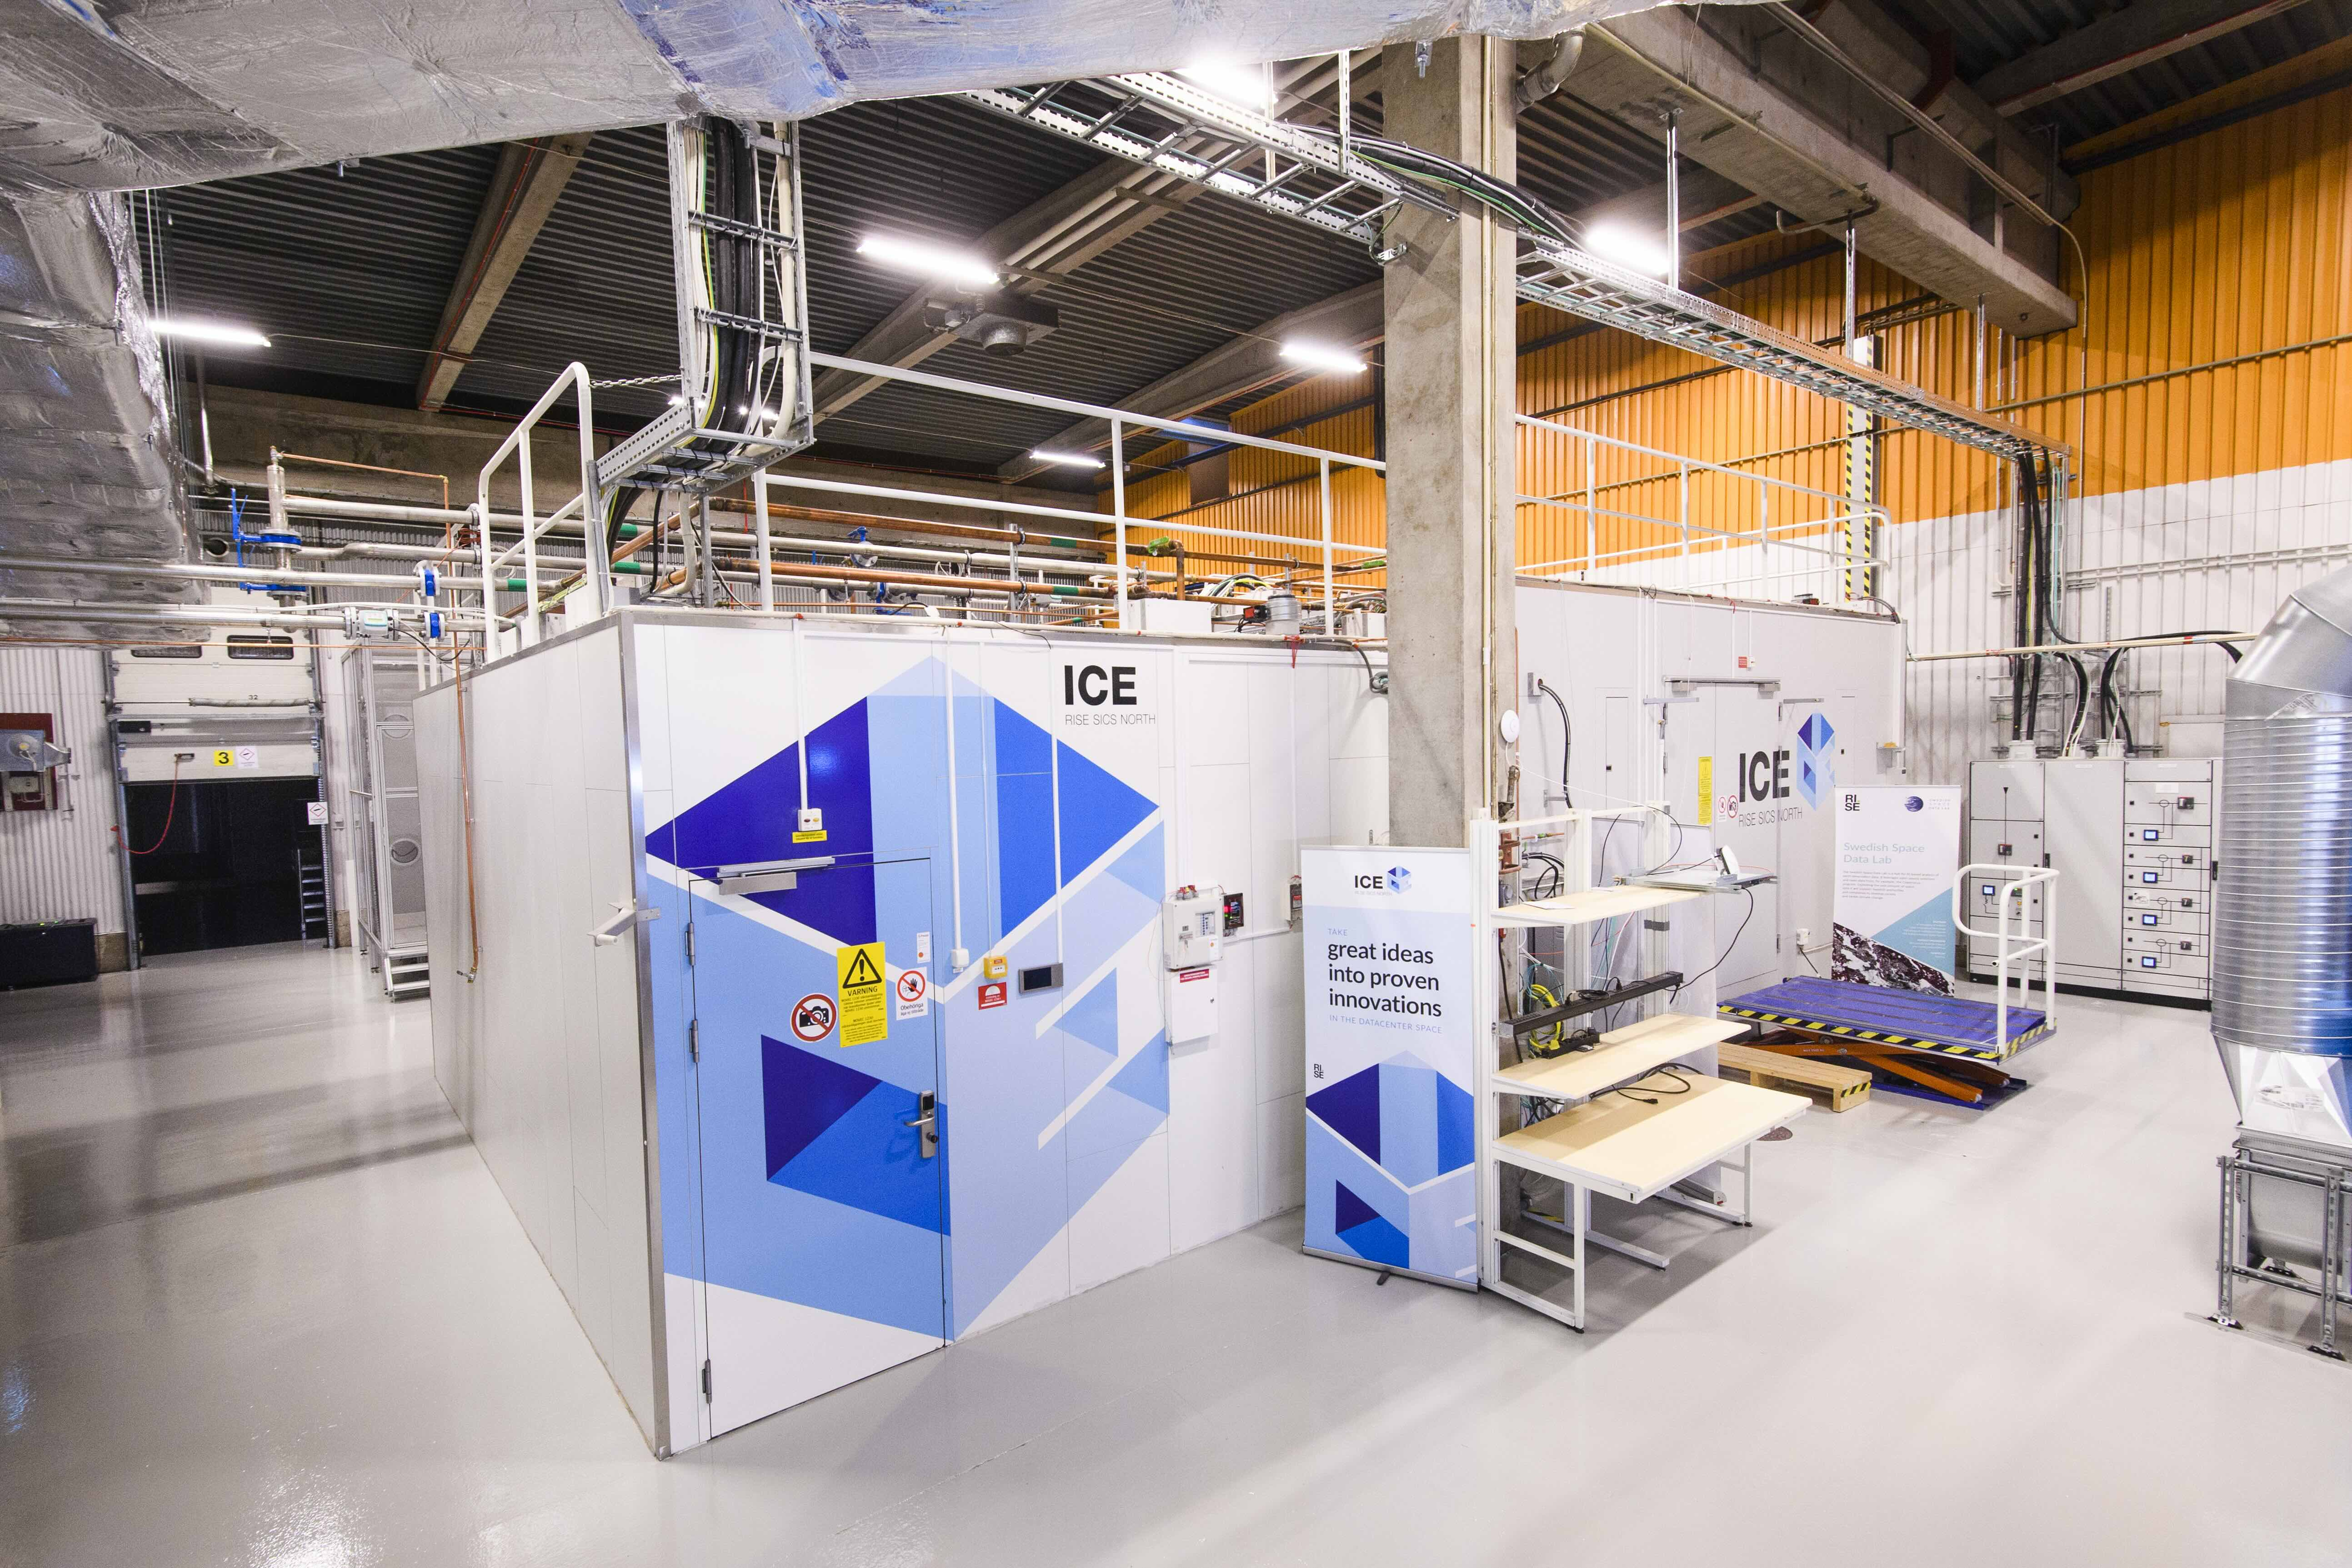
\includegraphics[width=\linewidth,height=38mm,keepaspectratio]
        {../heatwise-thermal-twin/images/datacenter.jpeg}
      \par\smallskip
      {\small\color{rwth-blue-100}\textbf{RISE ICE Datacenter research facility,\\Lule\aa{}, Sweden.}}
    \column{0.41\textwidth}
      \hspace*{-7mm}%
      \begin{minipage}[t]{\linewidth}
      \dataheading{The experiment}
      \small
      \begin{itemize}
        \item \textbf{9 servers / 18 CPUs} in the RISE server wind tunnel.
        \item Two Intel Xeon E5-2678 v3 CPUs per server.
        \item Five air-cooling cases; values every 5 minutes.
      \end{itemize}
      \smallskip
      \textbf{Original study:} \\ thermal performance of air vs.\ two-phase chip cooling.
      \end{minipage}
  \end{columns}
  \medskip
  \begin{uncoverenv}<2->
  \begin{beamercolorbox}[sep=1.7mm,wd=\textwidth]{data panel}
    \small
    \begin{itemize}
      \setlength{\itemsep}{1pt}
      \vspace{-1.5mm}
      \item<2-> \textbf{Our inputs:} CPU power {\color{rwth-blue-100}$P$}, air inlet temperature {\color{rwth-blue-100}$T_{\mathrm{inlet}}$}, raw fan signal {\color{rwth-blue-100}$F$}.
      \item<3-> \textbf{Our output:} largest of the 18 CPU temperature averages over an approximately steady interval.
    \end{itemize}
    \vspace{-1.5mm}
  \end{beamercolorbox}
  \end{uncoverenv}
  \datasource{Photo: \href{https://www.ri.se/en/news/from-idea-to-an-internationally-recognised-innovation-environment-ice-datacenter-celebrates}{RISE / ICE Datacenter (2026)}.
    Data: \href{https://zenodo.org/records/23237930}{HEATWISE / Zenodo}; \href{https://doi.org/10.1016/j.csite.2026.107650}{Ebrahimpour Ahmadi et al., CSITE 78 (2026), 107650}.}
\end{frame}

% 4: 1:25--2:00. Reveals: simulated targets -> measurements -> future data.
\begin{frame}[more-space]{Introduction\enspace|\enspace Why start with measured data?}
  \vspace*{\fill}
  \begin{columns}[T,onlytextwidth]
    \column{0.48\textwidth}
      \begin{beamercolorbox}[sep=2.5mm,wd=\linewidth]{data panel}
        \dataheading{Simulator-generated targets}
        \small
        \begin{itemize}
          \item More points at chosen settings.
          \item Detailed CFD needs geometry / CAD and a fluid solver, e.g.\ OpenFOAM.
          \item Model assumptions add uncertainty.
        \end{itemize}
      \end{beamercolorbox}
    \column{0.49\textwidth}
      \begin{uncoverenv}<2->
      \begin{beamercolorbox}[sep=2.5mm,wd=\linewidth]{data panel}
        \dataheading{Experimental measurements}
        \small
        \begin{itemize}
          \item Fewer available points.
          \item Capture real heating and cooling physics.
          \item \textbf{Our choice for the first model.}
        \end{itemize}
      \end{beamercolorbox}
      \end{uncoverenv}
  \end{columns}
  \par\vfill
  \begin{uncoverenv}<3->
  \begin{beamercolorbox}[sep=2mm,wd=\textwidth]{data warning}
    \small
    \begin{itemize}
      \setlength{\itemsep}{1pt}
      \item The same workflow can use future simulated or measured data.
      \item More suitable data may help; \textbf{improvement still needs validation}.
    \end{itemize}
  \end{beamercolorbox}
  \end{uncoverenv}
  \datasource{Source: \href{https://www.openfoam.com/}{openfoam.com}}
\end{frame}

\section{Data and proposed methods}

% 5: 2:00--2:55. Reveals: graph/caption -> summary -> limits -> target box.
\begin{frame}[more-space]{Preprocessing: From time series to 19 observations}
  \begin{columns}[T,onlytextwidth]
    \column{0.69\textwidth}
      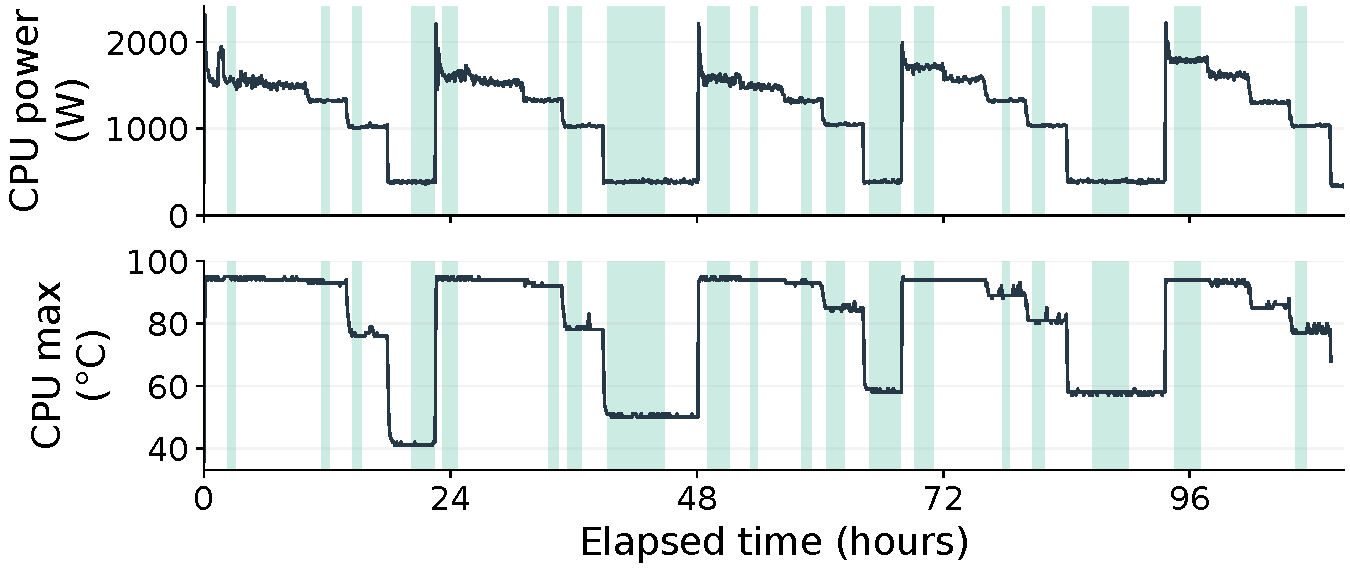
\includegraphics[width=\linewidth,height=44mm,keepaspectratio]{images/selection_readable.pdf}
      \par\smallskip
      {\small\color{selectiongreen}\textbf{One green band = one observation.}}
    \column{0.28\textwidth}
      \begin{uncoverenv}<2->
      \datametric{19}{approximately steady observations}
      \smallskip
      \small
      \begin{itemize}
        \setlength{\itemsep}{1pt}
        \item Wait after load changes.
        \item Keep stable periods with all 18 sensors.
        \item Average within each period.
      \end{itemize}
      \end{uncoverenv}
      \smallskip
      \begin{uncoverenv}<3->
      \begin{beamercolorbox}[sep=1.4mm,wd=\linewidth]{data limits}
        \small {\color{red!65!black}\textbf{Limits:}} sparse data, input dependency and throttling
      \end{beamercolorbox}
      \end{uncoverenv}
  \end{columns}
  \smallskip
  \begin{uncoverenv}<4->
  \begin{beamercolorbox}[sep=1.7mm,wd=\textwidth]{data panel}
    \small
    \begin{itemize}
      \setlength{\itemsep}{1pt}
      \vspace{-1.5mm}
      \item \textbf{Target:} largest of the 18 CPU temperature averages.
      \item This is a settled-temperature model, not a model of short temperature peaks.
    \end{itemize}
    \vspace{-1.5mm}
  \end{beamercolorbox}
  \end{uncoverenv}
  \datasource{Data limits: \hyperlink{backup-A2}{\textbf{A2}}--\hyperlink{backup-A3}{\textbf{A3}};
    full rules: \hyperlink{backup-A5}{\textbf{A5}}; threshold sensitivity: \hyperlink{backup-A7}{\textbf{A7}}.}
\end{frame}

% 6: 2:55--4:00. Reveals: model -> degree choice -> benefits -> reference.
\begin{frame}[more-space]{Polynomial Chaos Expansion}
  \begin{beamercolorbox}[sep=3mm,wd=\textwidth]{data panel}
    \centering
    \small A compact polynomial temperature model
    \[
      \widehat T_{\max}^{\mathrm{ss}}(\mathbf x)
        =\sum_{|\boldsymbol\alpha|\leq p}c_{\boldsymbol\alpha}\,
          \Psi_{\boldsymbol\alpha}(\boldsymbol\xi)
    \]
    {\footnotesize\color{black!60}Fitted weights $c_{\boldsymbol\alpha}$ $\times$ polynomial terms $\Psi_{\boldsymbol\alpha}$.
    \par Scaled inputs $\boldsymbol\xi\in[-1,1]^3$; degree $p=1$ or $2$.\par}
  \end{beamercolorbox}
  \medskip
  \begin{columns}[T,onlytextwidth]
    \column{0.48\textwidth}
      \begin{uncoverenv}<2->
      \dataheading{Small enough to start}
      \small
      \begin{itemize}
        \setlength{\itemsep}{1pt}
        \vspace{-1.5mm}
        \item 4 or 10 coefficients for three inputs.
        \item We will choose the degree using training data.
      \end{itemize}
      \vspace{-1.5mm}
      \end{uncoverenv}
    \column{0.49\textwidth}
      \begin{uncoverenv}<3->
      \dataheading{Why PCE?}
      \small
      \begin{itemize}
        \setlength{\itemsep}{1pt}
        \vspace{-1.5mm}
        \item Fast evaluation.
        \item Mean, variance and input influence can be read from the coefficients.
      \end{itemize}
      \vspace{-1.5mm}
      \end{uncoverenv}
  \end{columns}
  \medskip
  \begin{uncoverenv}<4->
  \begin{beamercolorbox}[sep=1.7mm,wd=\textwidth]{data warning}
    \small
    \begin{itemize}
      \setlength{\itemsep}{1pt}
      \item Independent uniforms give equal weight across each input range.
      \item This defines the Legendre basis; \textbf{not real operating probabilities}.
    \end{itemize}
  \end{beamercolorbox}
  \end{uncoverenv}
  \datasource{Method: \href{https://www.uqlab.com/pce-user-manual}{UQLab PCE manual}. Software: \hyperlink{backup-B1}{\textbf{B1}}; bounds / scaling: \hyperlink{backup-B3}{\textbf{B3}}; conditioning: \hyperlink{backup-B4}{\textbf{B4}}.}
\end{frame}

% 7: 4:00--5:05. Reveals: introduction -> signs -> fit -> assumptions.
\begin{frame}[more-space]{Physics-Informed PCE: Add monotonicity constraints}
  \vspace*{2mm}
  \small
  \begin{itemize}
    \item Fit the same 19 measurements, while enforcing expected heating and cooling trends.
    \item \textbf{Goal}: to reduce the search space and improve the fit
  \end{itemize}
  \par\vfill
  \begin{columns}[T,onlytextwidth]
    \column{0.50\textwidth}
      \begin{uncoverenv}<2->
      \begin{beamercolorbox}[sep=2.5mm,wd=\linewidth]{data panel}
        \dataheading{Expected directions}
        \small
        \renewcommand{\arraystretch}{1.8}
        \begin{tabular}{@{}ll@{}}
          $\dfrac{\partial\widehat T}{\partial P}\geq0$ & More CPU power: no cooler\\ \vspace{1.2mm}
          $\dfrac{\partial\widehat T}{\partial T_{\mathrm{inlet}}}\geq0$ & Warmer inlet: no cooler\\ \vspace{1.2mm}
          $\dfrac{\partial\widehat T}{\partial F}\leq0$ & More fan cooling: no hotter
        \end{tabular}
      \end{beamercolorbox}
      \end{uncoverenv}
    \column{0.47\textwidth}
      \begin{uncoverenv}<3->
      \begin{beamercolorbox}[sep=2.5mm,wd=\linewidth]{data panel}
        \dataheading{Same fit, restricted shape}
        \[
          \min_{\mathbf c}\sum_{i\in\mathrm{train}}(\widehat T_i-y_i)^2
        \]
        {\small\centering subject to these derivative signs.\par}
        \medskip
        {\footnotesize\color{black!60}$y_i$: measured target.\par}
      \end{beamercolorbox}
      \end{uncoverenv}
  \end{columns}
  \par\vfill
  \begin{uncoverenv}<4->
  \begin{beamercolorbox}[sep=1.7mm,wd=\textwidth]{data panel}
    \small Derivatives easy to calculate because the PCE is a polynomial. The constrained fit is a \textbf{quadratic program}.
  \end{beamercolorbox}
  \end{uncoverenv}
\par\vfill
  \begin{uncoverenv}<5->
  \begin{beamercolorbox}[sep=1.7mm,wd=\textwidth]{data warning}
    \small These constraints are assumptions to test!
  \end{beamercolorbox}
  \end{uncoverenv}
  \datasource{Full fit: \hyperlink{backup-C1}{\textbf{C1}}; corner argument: \hyperlink{backup-C3}{\textbf{C3}}.}
\end{frame}

% 8: 5:05--6:00. Reveals: case diagram/steps -> comparison box.
\begin{frame}[more-space]{PCE vs PI-PCE: same basis, measurements and test cases}
  \vspace*{\fill}
  \noindent\makebox[\textwidth][c]{%
    \begin{tikzpicture}[
      node distance=3mm,
      block/.style={rounded corners=1mm,draw=rwth-blue-100!50,
        fill=rwth-blue-100!6,text width=22mm,minimum height=13mm,
        inner sep=2mm,align=center,font=\small}]
      \node[block,fill=casefour!12] (c1) {Case 1\\\textbf{Test}};
      \node[block,right=of c1] (c2) {Case 2\\Train};
      \node[block,right=of c2] (c3) {Case 3\\Train};
      \node[block,right=of c3] (c4) {Case 4\\Train};
      \node[block,right=of c4] (c5) {Case 5\\Train};
    \end{tikzpicture}%
  }
  \par\vfill
  \small
  \begin{enumerate}
    \item Hold out one complete case.
    \item Choose degree on the other four; refit and predict the held-out case.
    \item Repeat until all five cases have been tested.
  \end{enumerate}
  \par\vfill
  \begin{uncoverenv}<2->
  \begin{beamercolorbox}[sep=2mm,wd=\textwidth]{data panel}
    \small
    \begin{itemize}
      \setlength{\itemsep}{1pt}
      \item Compare \textbf{prediction error} and \textbf{heating / cooling trends}.
      \item Flag test settings outside the training ranges.
    \end{itemize}
  \end{beamercolorbox}
  \end{uncoverenv}
  \datasource{Full protocol: \hyperlink{backup-C4}{\textbf{C4}}.}
\end{frame}

% 9: 6:00--6:40. Reveals: moments -> Sobol indices -> uncertainty note.
\begin{frame}[more-space]{UQ and Sensitivity: What the coefficients tell us}
  \begin{columns}[T,onlytextwidth]
    \column{0.49\textwidth}
      \begin{beamercolorbox}[sep=2.5mm,wd=\linewidth]{data panel}
        \begin{minipage}[t][35mm][t]{\dimexpr\linewidth-5mm\relax}
          \dataheading{How much does temperature vary?}
          \[
            \mu=c_{\mathbf0},\qquad
            \sigma^2=\sum_{\boldsymbol\alpha\ne\mathbf0}c_{\boldsymbol\alpha}^2
          \]
          \small Mean and variance under the chosen input reference.
        \end{minipage}
      \end{beamercolorbox}
    \column{0.49\textwidth}
      \begin{uncoverenv}<2->
      \begin{beamercolorbox}[sep=2.5mm,wd=\linewidth]{data panel}
        \begin{minipage}[t][35mm][t]{\dimexpr\linewidth-5mm\relax}
          \dataheading{Which inputs matter most?}
          \small\raggedright
          \[
            S_i^{\mathrm T}=\frac{\sum_{\alpha_i>0}c_{\boldsymbol\alpha}^{2}}{\sigma^2},
            \qquad\sigma^2>0
          \]
          \begin{itemize}
            \item \textbf{First-order:} one input acting alone.
            \item \textbf{Total:} also includes interactions.
          \end{itemize}
          \smallskip
          \footnotesize Larger index = more influence, \textbf{for our assumed input distributions}.
        \end{minipage}
      \end{beamercolorbox}
      \end{uncoverenv}
  \end{columns}
  \medskip
  \begin{uncoverenv}<3->
  \begin{beamercolorbox}[sep=2mm,wd=\textwidth]{data warning}
    \small
    \begin{itemize}
      \setlength{\itemsep}{1pt}
      \item \textbf{Not prediction error.} Real operating uncertainty needs separate data.
      \item For uncertainty of max temperature w.r.t air inlet temperature, fix CPU / fan settings and rearrange the same PCE.
    \end{itemize}
  \end{beamercolorbox}
  \end{uncoverenv}
  \datasource{Method: \href{https://www.uqlab.com/pce-user-manual}{UQLab PCE manual}. Full Sobol formulas: \hyperlink{backup-B2}{\textbf{B2}}; conditional moments: \hyperlink{backup-D1}{\textbf{D1}}.}
\end{frame}

% 10: 6:40--7:25. Reveals: main workflow -> two other loops.
\begin{frame}[more-space]{The Proposed Digital Twin}
  \vspace*{\fill}
  \noindent\makebox[\textwidth][c]{%
    \begin{tikzpicture}[
      node distance=6mm,
      stage/.style={draw=rwth-blue-100!55,fill=rwth-blue-100!6,
        rounded corners=1.5mm,inner sep=2mm,text width=38mm,
        minimum height=19mm,align=center,font=\small},
      flow/.style={->,thick,rwth-blue-100,>={Latex[length=2mm]}}]
      \node[stage] (measure) {{\color{rwth-blue-100}\textbf{Measure}}\\[2mm]
        CPU temperatures,\\inlet temperature\\and current CPU / fan settings};
      \node[stage,right=of measure] (predict) {{\color{rwth-blue-100}\textbf{Predict}}\\[2mm]
        Maximum settled\\CPU temperature};
      \node[stage,right=of predict] (compare) {{\color{rwth-blue-100}\textbf{Compare and Actuate}}\\[2mm]
        CPU power $P$\\and cooling signal $F$};
      \draw[flow] (measure)--(predict);
      \draw[flow] (predict)--(compare);
    \end{tikzpicture}%
  }
  \par\vfill
  \begin{uncoverenv}<2->
  {\small\color{black}\textbf{Two other loops:}\par}
  \medskip
  \begin{columns}[T,onlytextwidth]
    \column{0.48\textwidth}
      \dataheading{Safety loop}
      \small Monitor temperatures; verified fallback.\\
      Hardware protection handles peaks.
    \column{0.48\textwidth}
      \dataheading{Slower learning loop}
      \small New steady data $\rightarrow$ refit $\rightarrow$ validate.
  \end{columns}
  \end{uncoverenv}
  \datasource{Full definition: \hyperlink{backup-E1}{\textbf{E1}}; learning loop: \hyperlink{backup-E2}{\textbf{E2}};
    robust formulation: \hyperlink{backup-E3}{\textbf{E3}}.}
\end{frame}

% 11: 7:25--7:55. Reveals: current status -> transition arrow and backlog.
\begin{frame}[more-space]{Outlook}
  \begin{beamercolorbox}[sep=3mm,wd=\textwidth]{data panel}
    \begin{minipage}[t][24mm][t]{\dimexpr\textwidth-6mm\relax}
      \dataheading{Current status}
      \small
      \begin{itemize}
        \item Input analysis: 19 approximately steady observations.
        \item Model concept and assumptions.
        \item PCE vs PI-PCE comparison plan.
      \end{itemize}
    \end{minipage}
  \end{beamercolorbox}
  \par\nointerlineskip
  \begin{uncoverenv}<2->
  \hbox to\textwidth{\hfil
    \begin{tikzpicture}
      \path[use as bounding box] (-4mm,-4mm) rectangle (4mm,4mm);
      \draw[-{Latex[length=3mm,width=3.5mm]},line width=2pt,rwth-blue-100]
        (0,3mm)--(0,-3mm);
    \end{tikzpicture}%
    \hfil}
  \nointerlineskip
  \begin{beamercolorbox}[sep=3mm,wd=\textwidth]{data warning}
    \begin{minipage}[t][20mm][t]{\dimexpr\textwidth-6mm\relax}
      \dataheading{Backlog for next steps}
      \small
      \begin{itemize}
        \item Fit and compare PCE vs PI-PCE.
        \item Report errors and reference sensitivity.
        \item Update digital twin concept if needed.
      \end{itemize}
    \end{minipage}
  \end{beamercolorbox}
  \end{uncoverenv}
\end{frame}

% 12: 7:55--8:00
\begin{frame}[c]
  \centering
  {\color{rwth-blue-100}\fontsize{25}{30}\selectfont\bfseries Thanks for listening!\par}
  \vspace{5mm}
  {\color{black!65}\large Questions and discussion\par}
\end{frame}
